\documentclass[aspectratio=169,onlytextwidth]{beamer}
%% Choose aspect ratio:
% [aspectratio=43]  % 4:3 (default)
% [aspectratio=169] % 16:9, wide


% preamble {{{ %
\usetheme[standard,]{tugraz2018}
%% Choose main theme variant:
% [standard]        % standard (default)
% [institute]       % with institute's graphical acronym on the left
% [minimal]         % with reduced visuals

%% Choose your font style:
%                   % Helvetica (default for Corporate Design)
% [webfont]         % Source Sans Pro (as used on tugraz.at)
% [nofont]          % no font loaded - Computer Modern Sans

%% Choose your department's color instead of TU Graz red (optional):
% [arch]            % 
% [bau]             %
% [etit]            %
% [mbww]            %
% [tcvp]            %
% [mpug]            %
% [infbio]          %


\usepackage[utf8]{inputenc}
\usepackage[english]{babel}
%% Choose your language:
% [ngerman]   % German
% [english]   % English


%% Add your own packages, macros, etc.
\graphicspath{{figures/}}
\usepackage{booktabs}
\usepackage{colortbl}
\usepackage{csquotes}

%% Enter presentation metadata
\setbeamerfont{title}{size=\Large}
\title[mCPT at SemEval-2023 Task 3]{Multilingual Label-Aware Contrastive\\Pre-Training of Transformers for Few- and Zero-shot Framing Detection}
\author{Markus Reiter-Haas \and Alexander Ertl \and Kevin Innerhofer \and Elisabeth Lex}
\date{Graz, July 2023}
\institute{ISDS}
\instituteurl{www.isds.tugraz.at}

%% Logos
\institutelogo{beamerthemetugraz/institute/ISDS}  % graphical acronym for [institute] theme (left margin)
% \additionallogo{figures/logo}  % additional institute/department logo (footline; optional)
% \logobar{Supported by: ...}  % sponsors (titlepage; optional)
% }}} preamble %


\begin{document}

\begin{frame}[plain]
  \maketitle
\end{frame}


\begin{frame}{Outline}
  \tableofcontents
\end{frame}


% Introduction {{{ %
\section{Introduction}

\begin{frame}{Desiderata}
  \begin{columns}[T]
    \column{0.5\textwidth}
      Approach that handles
      \begin{itemize}
        \item Multi-label few-shot setting
        \item Imbalanced datasets
        \item Shifts in distribution
      \end{itemize}
  
    \column{0.5\textwidth}
      \vspace{-1.4cm}
      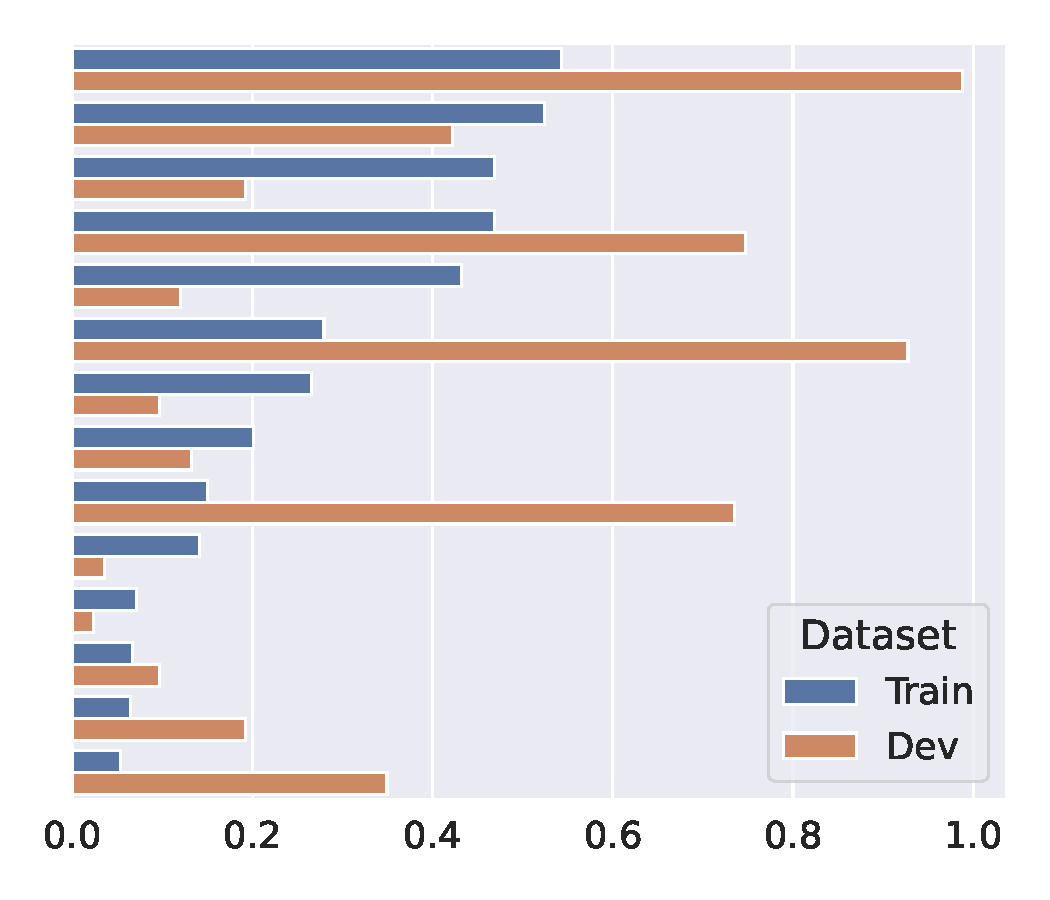
\includegraphics[height=.8\textheight]{imbalances_train_dev}
  \end{columns}
\end{frame}
% }}} Introduction %


% mCPT {{{ %
\section{Multilingual Contrastive Pre-Training (mCPT)}

\begin{frame}{The mCPT Pipeline}
  \centering
  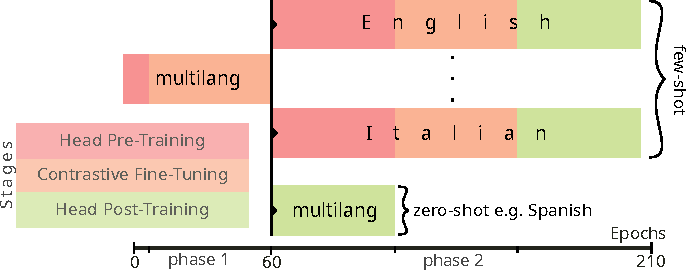
\includegraphics[height=0.6\textheight]{pipeline}
\end{frame}

\begin{frame}{Label-Aware Contrastive Learning}
  \centering
  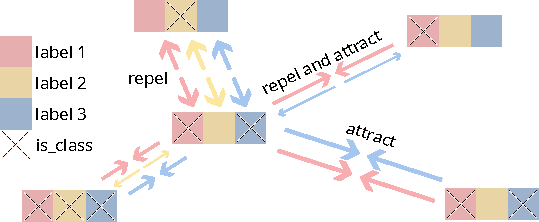
\includegraphics[height=0.6\textheight]{contrast}
\end{frame}

\begin{frame}{HeroCon Loss\footnotemark}
  \begin{columns}[T]
    \column{0.6\textwidth}
      \begin{itemize}
        \item Multi-Component loss function
        \item Positive pairs should be similar
        \item Negative pairs should be dissimilar
        \item Weighted by Hamming distance
      \end{itemize}

    \column{0.4\textwidth}
      \begin{equation*}
        \mathcal{L} = \mathcal{L}_{BCE} + \alpha \mathcal{L}_{CON}
      \end{equation*}
      \begin{equation*}
        \mathcal{L}_{BCE} = \text{binary cross-entropy}
      \end{equation*}
      \begin{equation*}
        \mathcal{L}_{CON} = \text{contrastive}
      \end{equation*}
  \end{columns}

  \footnotetext[1]{\scriptsize Zheng, L., Xiong, J., Zhu, Y., \& He, J. (2022, August). Contrastive learning with complex heterogeneity. In Proceedings of the 28th ACM SIGKDD Conference on Knowledge Discovery and Data Mining (pp. 2594-2604).}
\end{frame}

\begin{frame}{Contrast Sampling}
  \begin{itemize}
    \item Loss function computed on batches
      \begin{itemize}
        \item at least one sample per class for negative pairs
        \item at least two samples per class for positive pairs
      \end{itemize}
    \item Implicitly performs oversampling
  \end{itemize}
\end{frame}

\begin{frame}{The mCPT Pipeline}
  \centering
  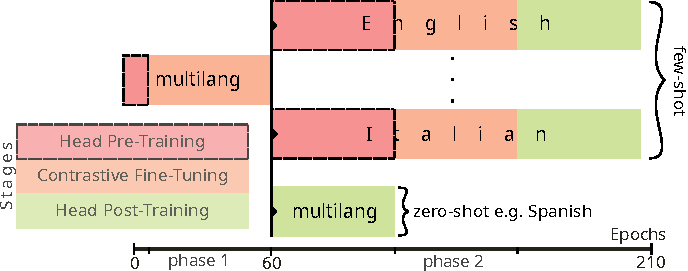
\includegraphics[height=0.6\textheight]{pipeline_hlpretrain}
\end{frame}

\begin{frame}{The mCPT Pipeline}
  \centering
  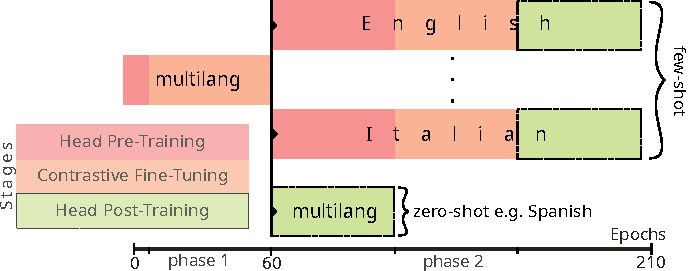
\includegraphics[height=0.6\textheight]{pipeline_hlposttrain}
\end{frame}
% }}} mCPT %


% Results {{{ %
\section{Results}

\begin{frame}{Ablation Study}
  \centering
  \begin{tabular}{l c c c c c c c} \toprule
    Model & en & it & ru & fr & ge & po & $\overline{\Delta}$  \\ \midrule
    \rowcolor[gray]{.9} \emph{mCPT}+CS & \textbf{.688} & \textbf{.590} & .519 & \textbf{.575} & \textbf{.591} & .638 &  \\
    - CS\footnotemark[1] & .682 &  .585 & \textbf{.520} & .570 & .561 & .636 & -.008 \\
    - PT\footnotemark[2] & .681 & .545 & .475 & .563 & .583 & .616 & -.015 \\
    - $\mathcal{L}_{CON}$ & .657 & .521 & .436 & .524 & .570 & \textbf{.645} & -.018 \\
    - E2E\footnotemark[3] & .629 & .519 & .500 & .535 & .586 & .633 & .008 \\
    \bottomrule
  \end{tabular}
  \vfill
  \footnoterule \footnotesize
  \begin{minipage}[b]{\textwidth}
    \textsuperscript{1} contrast-sampling \hspace{0.3cm}
    \textsuperscript{2} multilingual pre-training \hspace{0.3cm}
    \textsuperscript{3} end-to-end training
  \end{minipage}
\end{frame}

\begin{frame}{Embeddings}
  \begin{columns}[T]
    \column{0.3\textwidth}
      $\mathcal{L}_{CON}$ optimizes \footnotemark[1]
      \begin{itemize}
        \item Uniformity
        \item Alignment
      \end{itemize}

    \column{0.7\textwidth}
      \vspace{-1.9cm}
      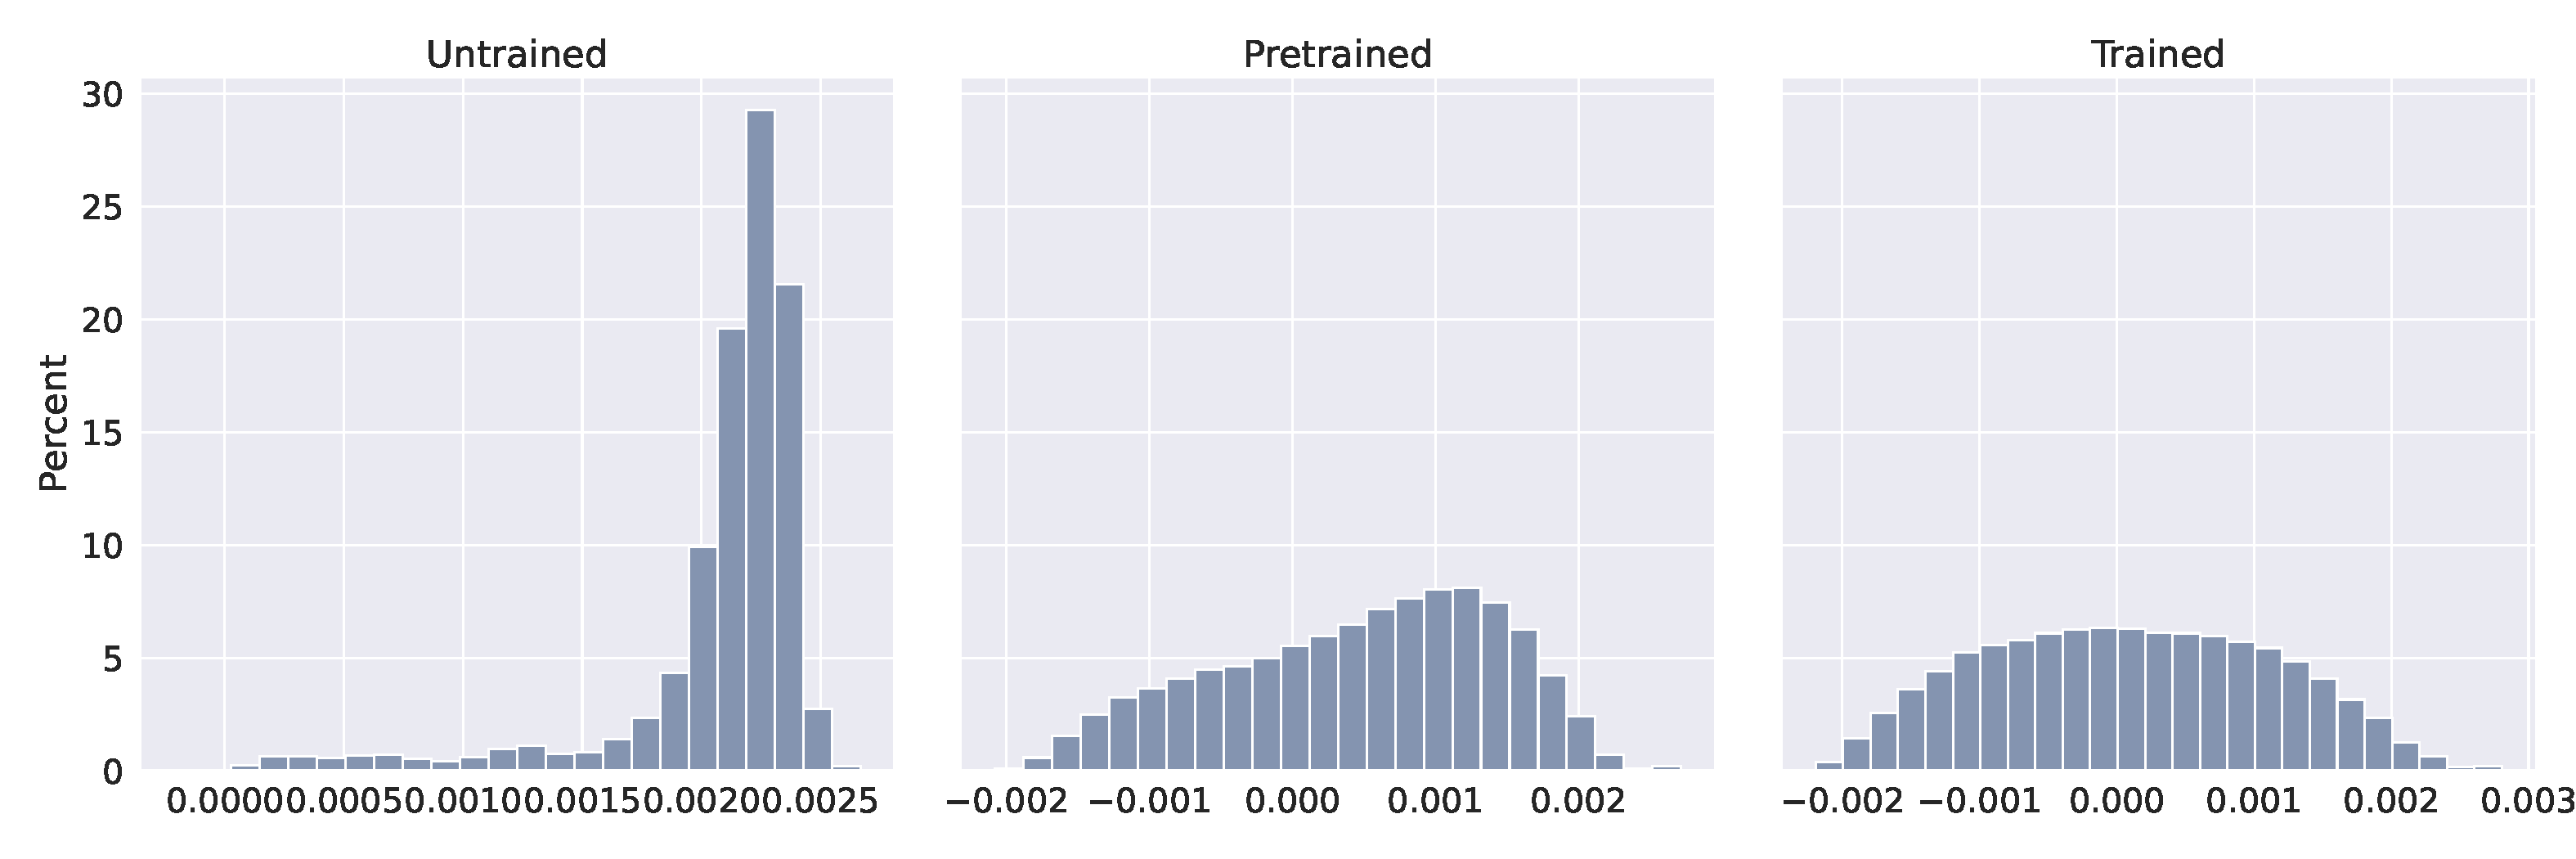
\includegraphics[width=\textwidth]{uniformity}
      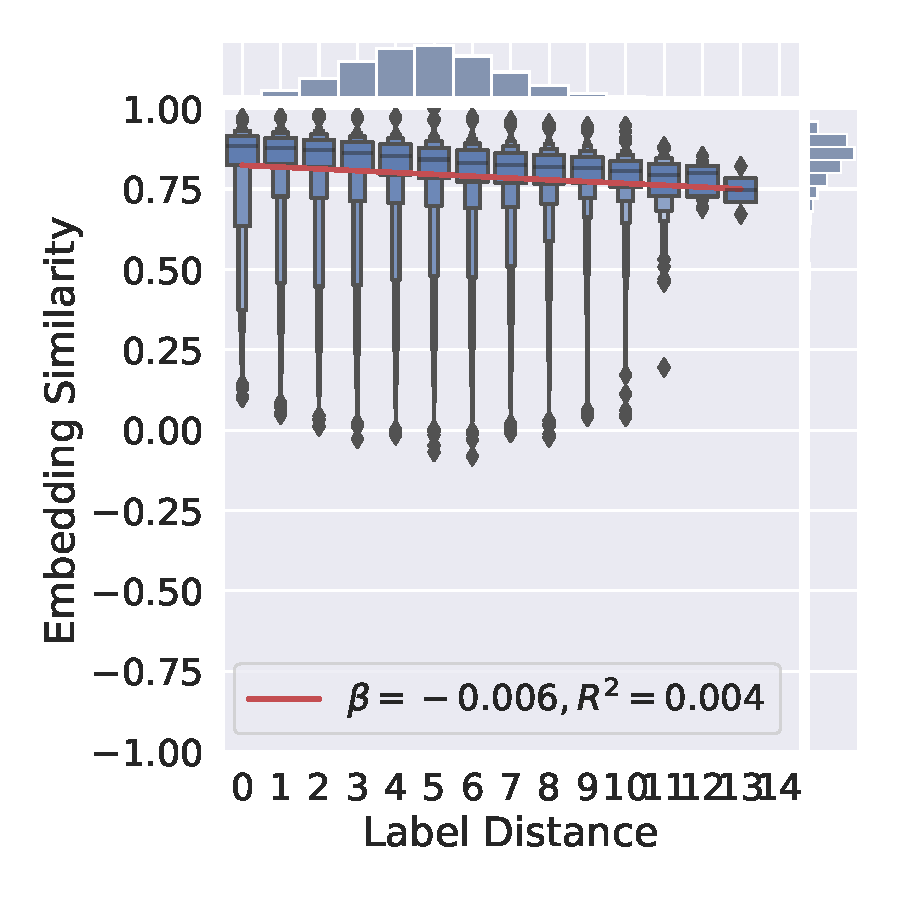
\includegraphics[width=0.32\textwidth]{label_embedding_untrained}
      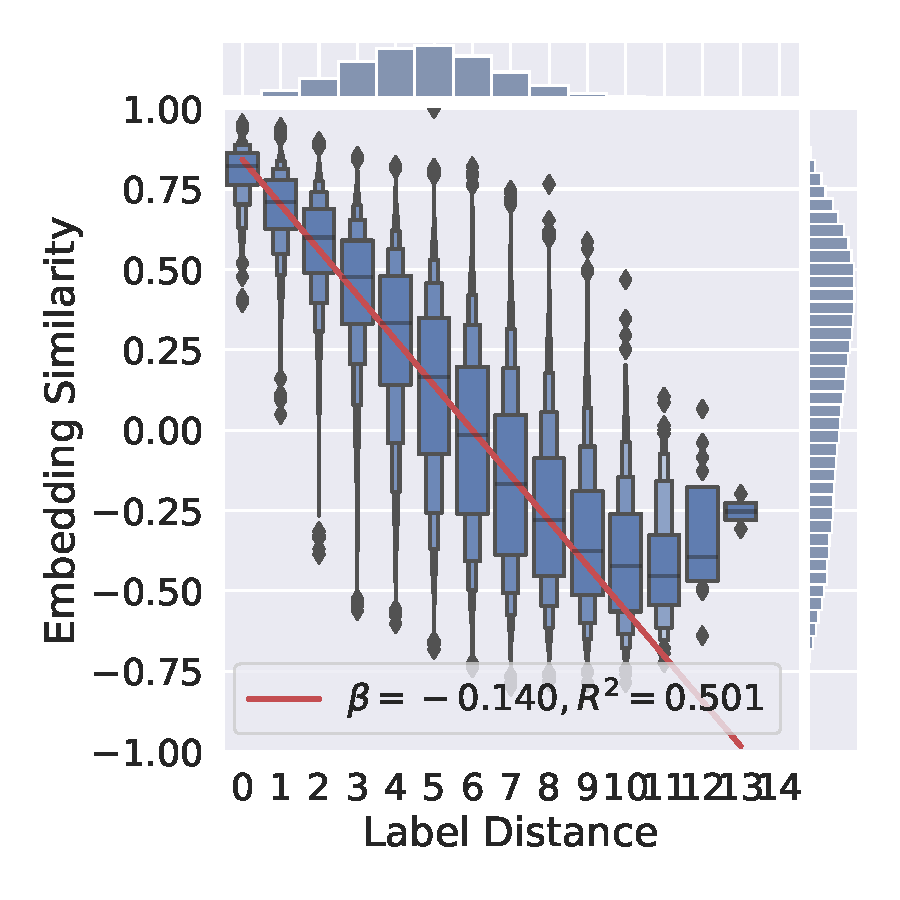
\includegraphics[width=0.32\textwidth]{label_embedding_pretrained}
      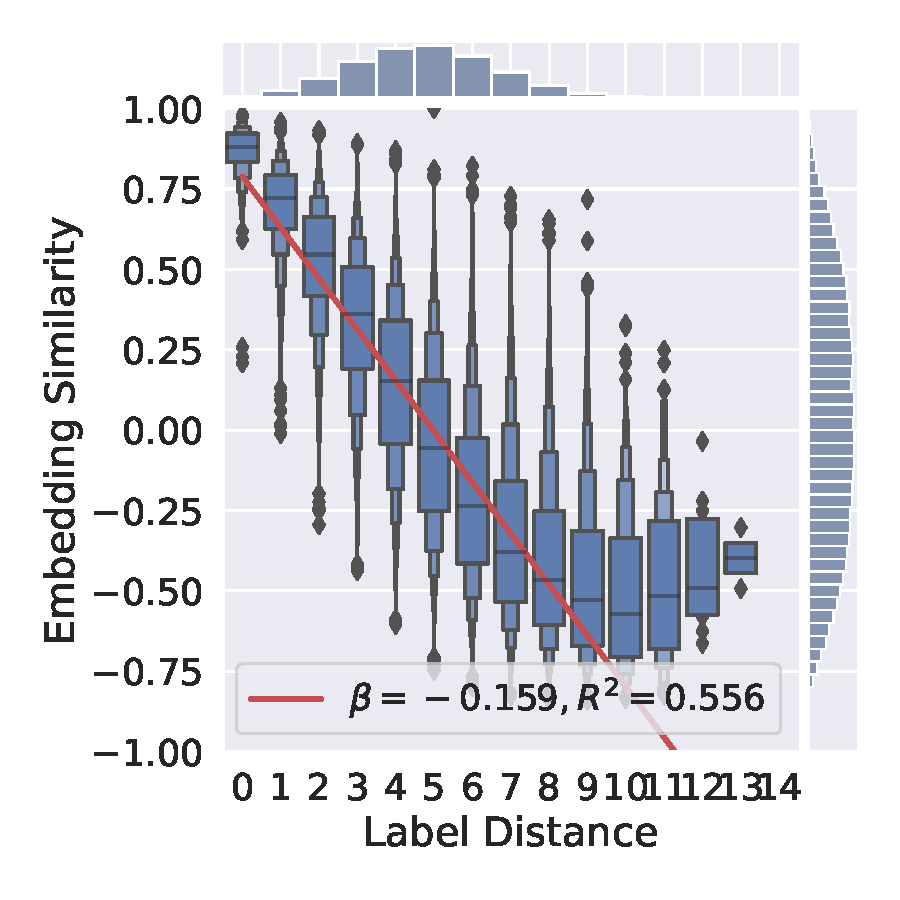
\includegraphics[width=0.32\textwidth]{label_embedding_trained}
  \end{columns}

  \vfill
  \footnoterule \tiny
  \begin{minipage}[b]{\textwidth}
    \textsuperscript{1} Wang, T. and Isola, P. (2020). Understanding Contrastive Representation Learning through Alignment and Uniformity on the Hypersphere. In International Conference on Machine Learning, pages 9929–9939.
  \end{minipage}
\end{frame}
% }}} Results %


\section{Conclusion}
\begin{frame}{Conclusion}
  \begin{block}{Multilingual Pre-Training}
    effectively increases the available amount of training data
  \end{block}
  \begin{block}{Contrastive Learning}
    acts as a regularizer optimizing for uniformity and alignment in multi-label settings
  \end{block}
\end{frame}

\begin{frame}[c,plain]
  \centering
  \vspace{3cm}
  \Large Thank You for Your Attention
  \vspace{1cm}

  \begin{table}[b]
    \centering
    \small
    \renewcommand{\arraystretch}{2}
    \begin{tabular}{c l}
      \raisebox{-.3\height}{
\includegraphics[height=.6cm]{github}} &  \url{https://github.com/socialcomplab/semeval23-mcpt} \\
      \raisebox{-.3\height}{
\includegraphics[height=.6cm]{arxiv}}  & \url{https://arxiv.org/abs/2303.09901} \\
    \end{tabular}
  \end{table}
\end{frame}


\end{document}
